\documentclass[11pt, a4paper, spanish, openright, twoside]{book}
\usepackage[spanish, activeacute]{babel}
\usepackage[utf8]{inputenc}
%\usepackage[top=2.5cm, bottom=2.5cm, outer=1.75cm, inner=1.75cm, heightrounded, marginparwidth=2.5cm, marginparsep=0.3cm]{geometry}	%márgenes empequeñecidos
\usepackage[top=2.95cm, bottom=2.25cm, outer=2.75cm, inner=2.75cm, heightrounded, marginparwidth=2.5cm, marginparsep=0.3cm]{geometry}	%márgenes originalmente
\usepackage{dpg}
\usepackage{fli}

\usepackage{pgf}
\usepackage{tikz}

\usepgflibrary{shapes.geometric} % LATEX and plain TEX and pure pgf
\usetikzlibrary{arrows,automata,positioning}
\tikzstyle{accepting by double}= [double distance=1.6pt,double,outer sep=.5\pgflinewidth+.8pt] % esto es algo estético.
\renewcommand\shorthandsspanish{}  % para compatibilizar spanish con tikz

%%%%%%		Figuras		%%%%%%%%%%%%%%%%%%%
\usepackage[vflt]{floatflt}		%Entorno float-figure

%%%%%%		Page style		%%%%%%%%%%%%%%%%%%%
\renewcommand{\thepage}{\arabic{page}}% Arabic page numbers\fancyhead{}
\pagestyle{fancy}
\fancyfoot{}
\fancyhead[LO,RE]{Práctica 2}	%encabezado de pares: nombre de la sección
\fancyfoot[LE,RO]{\thepage}	%abajo a izqda en pares, derecha en impares: numero de pagina
%\fancyhead[LE]{\nouppercase{\leftmark}} %cuadro izquierdo de pagina par: parte y contador
\fancyfoot[CE]{Inteligencia Artificial} 
\fancyfoot[CO]{Doble Grado Informática-Matemáticas - Universidad Complutense}
\renewcommand{\footrulewidth}{0.4pt}
\renewcommand{\headrulewidth}{0.4pt}		% linea por debajo del encabezado
\renewcommand{\sectionmark}[1]{\markright{\textbf{\thesection. #1}}}	%negrita
\renewcommand{\labelitemi}{$\circ$} %Primer itemize con circunferencia vacia
\renewcommand{\labelitemii}{} %Segundo itemize con punto pequeño \cdot
\renewcommand*{\thesection}{\arabic{section}}	% Hace que no apareca el indice de capitulos y que comience en section

%%%%%%		Others		%%%%%%%%%%%%%%%%%%%
\setlength{\leftmarginii}{0em} %Segundo itemize sin sangria
\setlength{\leftmarginiii}{1em} %Tercer itemize casi sin sangria
\renewcommand{\labelitemiii}{ }
\pagenumbering{roman}
\addto{\captionsspanish}{\renewcommand*{\contentsname}{Índice}} %Cambia "Indice general" por "Indice"



\begin{document} 
\title{\Huge{\textsc{Inteligencia Artificiall}} \\
	\vspace{0.7cm}
	 \textsc{\Large{Práctica 2}} \\
	\vspace{1.5cm}
	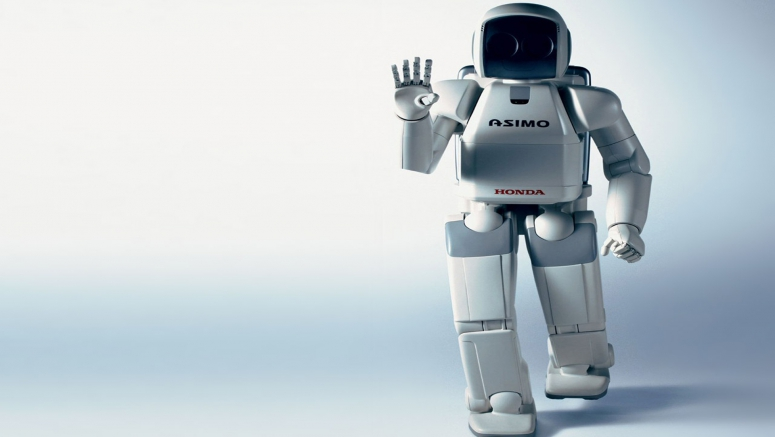
\includegraphics[scale=0.45]{robotHonda}}
\author{Enrique Ballesteros Horcajo\\
	Ignacio Iker Prado Rujas}
\date{\Today}
\maketitle

\newpage
\mbox{}
\thispagestyle{empty}						% Hoja en blanco, sin numeros ni nada
\newpage


\tableofcontents 							%INDICE hipervinculado

\newpage
\mbox{}
\thispagestyle{empty}						% Hoja en blanco, sin numeros ni nada
\newpage

\pagenumbering{arabic}						% Pone el contador de paginas a 1 y ahora en numeros normales

\vspace{3cm}


\newpage



\begin{section}{AimaDemoApp }


\end{section}

\begin{section}{Puzle de 8}

	
\end{section}

\begin{section}{Mapa desde Arad a Bucharest}
SLD es la heurística de línea recta, que elige la ciudad que está más cerca en línea recta del objetivo.

\end{section}


\begin{section}{SearchDemoOsmAgentApp }


\end{section}


\begin{section}{Librerías y definiciones de estado para el puzzle de 8 }


\end{section}


\begin{section}{Librerías y definiciones de estado para el mapa }


\end{section}

	
\section{Conclusiones}


	
\begin{thebibliography}{9}

\bibitem{aima}
	Russell, S.; Norvig, P, \\
	\emph{Artificial Intelligence, a modern aproach}.\\
	New Jersey: Pearson, 2010.

\end{thebibliography}


\end{document}

